% !TeX program = xelatex
% Original cover typography, logo, signatures and coordinates are retained.
% Reuse: change the following three commands for another laboratory work.
\documentclass{article}
\usepackage[paperwidth=595.3bp,paperheight=841.9bp,margin=0pt]{geometry}
\usepackage{fontspec}
\setmainfont{Times New Roman}
\usepackage{graphicx,eso-pic,tikz}
\newcommand{\LabNumber}{2}
\newcommand{\LabTitleFirst}{Архитектурные inductive biases в компьютерном зрении}
\newcommand{\LabTitleSecond}{augmentation, transfer и distribution shift}
\newcommand{\CoverText}[4]{%
  \node[anchor=base,inner sep=0pt,font=\fontsize{#3bp}{17bp}\selectfont]
    at ([xshift=#1bp,yshift=-#2bp]current page.north west) {#4};}
\pagestyle{empty}
\begin{document}
\AddToShipoutPictureBG*{\AtPageLowerLeft{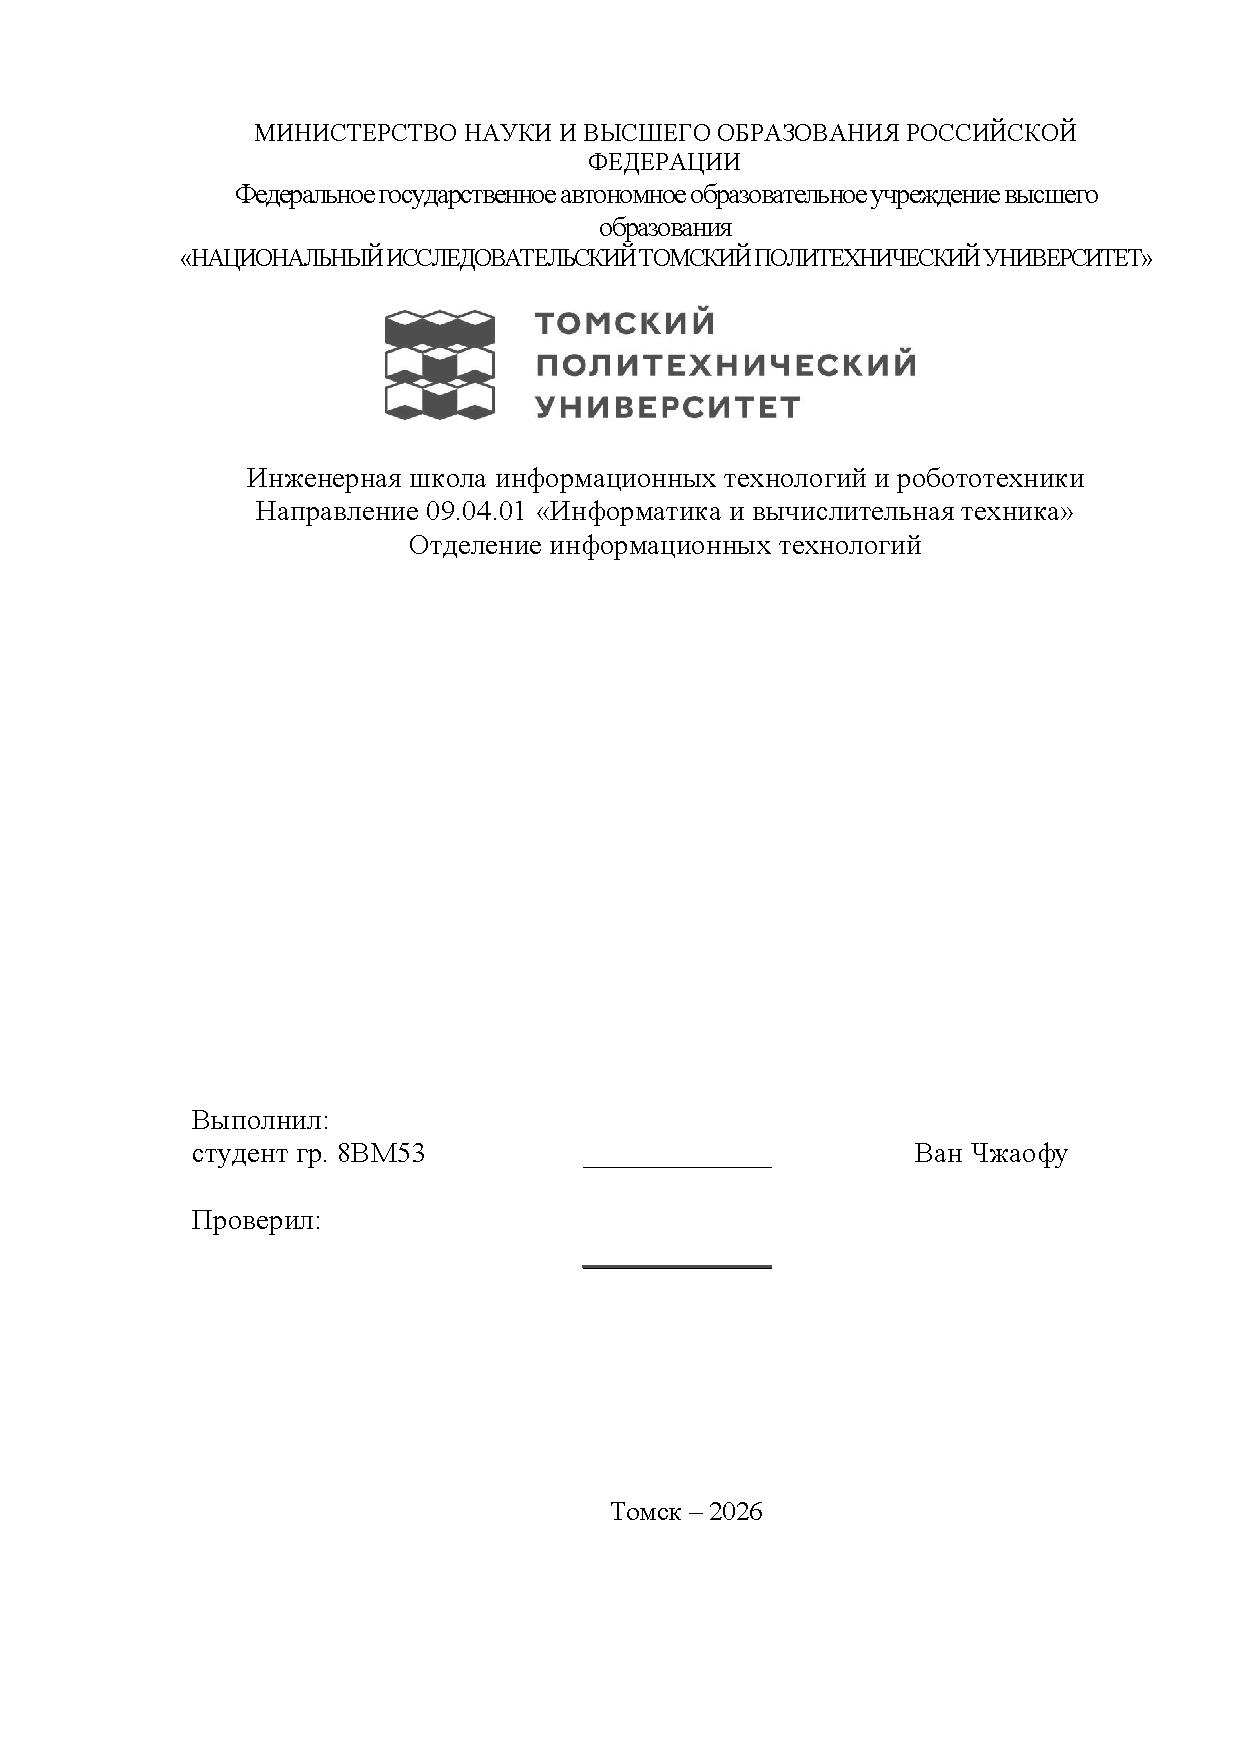
\includegraphics[width=595.3bp,height=841.9bp]{assets/title_base.pdf}}}
\AddToShipoutPictureFG*{%
\begin{tikzpicture}[remember picture,overlay]
\CoverText{319.5}{362.33}{14.05}{Лабораторная работа № 2}
\CoverText{319.5}{383}{13.5}{«Архитектурные inductive biases в компьютерном зрении}
\CoverText{319.5}{400}{13.5}{CNN vs Vision Transformer: sample efficiency,}
\CoverText{319.5}{417}{13.5}{augmentation, transfer и distribution shift»}
\CoverText{319.5}{457}{14.05}{по дисциплине «Нейронные сети»}
\CoverText{477.0}{606.29}{14.05}{Григорьев Д. С.}
\end{tikzpicture}}
\null
\end{document}
